% Copyright 2018-2022 FIUS
%
% This file is part of theo-vorkurs-folien.
%
% theo-vorkurs-folien is free software: you can redistribute it and/or modify
% it under the terms of the GNU General Public License as published by
% the Free Software Foundation, either version 3 of the License, or
% (at your option) any later version.
%
% theo-vorkurs-folien is distributed in the hope that it will be useful,
% but WITHOUT ANY WARRANTY; without even the implied warranty of
% MERCHANTABILITY or FITNESS FOR A PARTICULAR PURPOSE.  See the
% GNU General Public License for more details.
%
% You should have received a copy of the GNU General Public License
% along with theo-vorkurs-folien.  If not, see <https://www.gnu.org/licenses/>.

% !TeX program = pdflatex
% !TeX spellcheck = de
% Copyright 2018-2022 FIUS
%
% This file is part of theo-vorkurs-folien.
%
% theo-vorkurs-folien is free software: you can redistribute it and/or modify
% it under the terms of the GNU General Public License as published by
% the Free Software Foundation, either version 3 of the License, or
% (at your option) any later version.
%
% theo-vorkurs-folien is distributed in the hope that it will be useful,
% but WITHOUT ANY WARRANTY; without even the implied warranty of
% MERCHANTABILITY or FITNESS FOR A PARTICULAR PURPOSE.  See the
% GNU General Public License for more details.
%
% You should have received a copy of the GNU General Public License
% along with theo-vorkurs-folien.  If not, see <https://www.gnu.org/licenses/>.

\documentclass[aspectratio=43,10pt]{beamer}

\usetheme[progressbar=frametitle]{metropolis}
\usepackage{appendixnumberbeamer}
\usepackage[ngerman]{babel}
\usepackage[utf8]{inputenc}
%\usepackage{t1enc}
\usepackage[T1]{fontenc}
\usepackage[sfdefault,scaled=.85,lf]{FiraSans}
\usepackage{newtxsf}

\usepackage{booktabs}
\usepackage[scale=2]{ccicons}
\usepackage{hyperref}

\usepackage{pgf}
\makeatletter
\@ifclasswith{beamer}{notes}{
  \usepackage{pgfpages}
  \setbeameroption{show notes on second screen}
}{}
\makeatother
\usepackage{tikz}
\usetikzlibrary{arrows,automata,positioning}
\usepackage{pgfplots}
\usepgfplotslibrary{dateplot}

\usepackage{xspace}
\newcommand{\themename}{\textbf{\textsc{metropolis}}\xspace}

\usepackage{blindtext}
\usepackage{graphicx}
\usepackage{subcaption}
\usepackage{comment}
\usepackage{mathtools}
\usepackage{amsmath}
\usepackage{centernot}
\usepackage{amssymb}
\usepackage{proof}
\usepackage{tabularx}
\renewcommand{\figurename}{Abb.}
\usepackage{marvosym}
\usepackage{mathtools}
\usepackage{qrcode}
\usepackage{advdate}

\newcommand\daynr{0}

\definecolor{ExColor}{HTML}{17819b}

\newcommand{\emptyWord}{\varepsilon}
\let \emptyset\varnothing
\newcommand{\SigmaStern}{\Sigma^{*}}
\newcommand{\absval}[1]{|#1|}
\newcommand{\defeq}{\vcentcolon=}
\newcommand{\eqdef}{=\vcentcolon}
\newcommand{\nimplies}{\centernot\implies}

\newcommand{\naturals}{\ensuremath{\mathbb{N}}}
\newcommand{\integers}{\ensuremath{\mathbb{Z}}}
\newcommand{\rationals}{\ensuremath{\mathbb{Q}}}
\newcommand{\reals}{\ensuremath{\mathbb{R}}}
\newcommand{\iffspace}{\ensuremath{\iff\;}}

\setbeamertemplate{footline}[text line]
{\parbox{\linewidth}{Fachgruppe Informatik\hfill\insertpagenumber\hfill Vorkurs Theoretische Informatik\vspace{0.2in}}}

\newcommand{\Center}[1]{
  \begin{frame}<handout:0>[standout]
    #1
  \end{frame}
}

% Fix section pages in appendix
\AtBeginDocument{%
  \apptocmd{\appendix}{%
    \setbeamertemplate{section page}[simple]%
  }{}{}
}

\addtobeamertemplate{block begin}{}{\vskip 0em}
\addtobeamertemplate{block alerted begin}{}{\vskip 0em}
\addtobeamertemplate{block example begin}{}{\vskip 0em}

% Copyright 2018-2022 FIUS
%
% This file is part of theo-vorkurs-folien.
%
% theo-vorkurs-folien is free software: you can redistribute it and/or modify
% it under the terms of the GNU General Public License as published by
% the Free Software Foundation, either version 3 of the License, or
% (at your option) any later version.
%
% theo-vorkurs-folien is distributed in the hope that it will be useful,
% but WITHOUT ANY WARRANTY; without even the implied warranty of
% MERCHANTABILITY or FITNESS FOR A PARTICULAR PURPOSE.  See the
% GNU General Public License for more details.
%
% You should have received a copy of the GNU General Public License
% along with theo-vorkurs-folien.  If not, see <https://www.gnu.org/licenses/>.



% Configuration for slides

% The date of the first day of the Theo-Vorkurs in Format dd/mm/yyyy
\SetDate[10/10/2022]

% Invite URL to the Ersti-Telegram-Group. Used for text on slide as well as QR-Code
\newcommand\telegramurl{https://t.me/+Q92w5biyY903NjEy}

% The url to the handout of the current day with the current day as argument. Used for the qr-code in the slides. 
\newcommand{\handouturl}[1]{https://fius.de/wp-content/uploads/2022/10/day-#1-handout.pdf}


\renewcommand\daynr{1}
% Copyright 2018-2022 FIUS
%
% This file is part of theo-vorkurs-folien.
%
% theo-vorkurs-folien is free software: you can redistribute it and/or modify
% it under the terms of the GNU General Public License as published by
% the Free Software Foundation, either version 3 of the License, or
% (at your option) any later version.
%
% theo-vorkurs-folien is distributed in the hope that it will be useful,
% but WITHOUT ANY WARRANTY; without even the implied warranty of
% MERCHANTABILITY or FITNESS FOR A PARTICULAR PURPOSE.  See the
% GNU General Public License for more details.
%
% You should have received a copy of the GNU General Public License
% along with theo-vorkurs-folien.  If not, see <https://www.gnu.org/licenses/>.

\title{Vorkurs Theoretische Informatik}

\if\daynr1
    \subtitle{Einführung in die Grundideen, Mengenlehre und Aussagenlogik}
    \newcommand\daynamestr{Montag}
\fi
\if\daynr2
    \subtitle{Grundlagen der Beweise}
    \newcommand\daynamestr{Dienstag}
    \AdvanceDate
\fi
\if\daynr3
    \subtitle{Induktion und Einführung in die Grammatik}
    \newcommand\daynamestr{Mittwoch}
    \AdvanceDate\AdvanceDate
\fi
\if\daynr4
    \subtitle{Einführung in reguläre Sprachen}
    \newcommand\daynamestr{Donnerstag}
    \AdvanceDate\AdvanceDate\AdvanceDate
\fi
\if\daynr5
    \subtitle{Einführung in reguläre Sprachen}
    \newcommand\daynamestr{Freitag}
    \AdvanceDate\AdvanceDate\AdvanceDate
\fi


\date{\daynamestr, \today}

\author{Arbeitskreis Theo-Vorkurs}
\institute{Fachgruppe Informatik}
% \titlegraphic{\hfill\includegraphics[height=1.5cm]{logo.pdf}}

% \titlegraphic{\hfill\includegraphics[height=1.5cm]{logo.pdf}}

\begin{document}

\maketitle

\only<1|handout:0>{
	\setbeamercolor{background canvas}{bg=Bluecreen}
	\setbeamertemplate{title page}{
    \begin{minipage}[b][\paperheight]{\textwidth}
        \vspace{2em}
        \fontspec{Segoe UI}
        {
            \makeatletter
            \color{white}
            {\fontsize{40}{50}\selectfont
                :)
            }
            \par
            \vspace{1em}
            Your Studiengang ran into a problem and needs to be restructured.
            We're working on a \textbf{\inserttitle} for you.
            \par
            \vspace{.5em}
            \the\day .\the\month .\the\year\% complete
            % \ifx\inserttitle\@empty
            % \else\usebeamertemplate*{title}
            % \fi
            % \ifx\insertsubtitle\@empty
            % \else\usebeamertemplate*{subtitle}
            % \fi
            % \usebeamertemplate*{title separator}
            % \ifx\beamer@shortauthor\@empty
            % \else\usebeamertemplate*{author}
            % \fi
            % \ifx\insertdate\@empty
            % \else\usebeamertemplate*{date}
            % \fi
            % \ifx\insertinstitute\@empty
            % \else\usebeamertemplate*{institute}
            % \fi
            \par
            \vspace{2.5cm}
            \insertsubtitle
            \vfill
            {\fontsize{5pt}{5pt}\selectfont
                \insertauthor\ \textemdash\ \insertinstitute
            }
            \vspace{1.5em}
            \makeatother
        }
        \ifx\inserttitlegraphic\@empty
            \else{%
                \begin{tikzpicture}[remember picture,overlay]
                    \node[xshift=-10.5cm,yshift=-5cm] at (current page.north east){%
                        \colorbox{white}{
                            \only<1|handout:0>{
                                \qrcode[height=4em,padding]{\handouturl{\daynr}}
                            }
                        }};
                    \node[xshift=-8cm,yshift=-4.2cm] at (current page.north east){%
                        \small
                        \color{white}
                        Aktuelle Folien
                    };
                \end{tikzpicture}

            }
        \fi
    \end{minipage}
}
	\maketitle
	\setbeamercolor{background canvas}{
		use=palette primary,
		bg=palette primary.fg
	}
}

\metroset{sectionpage=progressbar,subsectionpage=none}

\section{Allgemeines}
% Copyright 2018-2022 FIUS
%
% This file is part of theo-vorkurs-folien.
%
% theo-vorkurs-folien is free software: you can redistribute it and/or modify
% it under the terms of the GNU General Public License as published by
% the Free Software Foundation, either version 3 of the License, or
% (at your option) any later version.
%
% theo-vorkurs-folien is distributed in the hope that it will be useful,
% but WITHOUT ANY WARRANTY; without even the implied warranty of
% MERCHANTABILITY or FITNESS FOR A PARTICULAR PURPOSE.  See the
% GNU General Public License for more details.
%
% You should have received a copy of the GNU General Public License
% along with theo-vorkurs-folien.  If not, see <https://www.gnu.org/licenses/>.

\subsection{Organisatorisches}
\begin{frame}[fragile]{Wer sind wir?}
    \begin{itemize}
        \item
            Fachgruppe Informatik
            \begin{itemize}
                \item Unser Ziel: \\
                Das Leben von uns Studis während des Studiums angenehmer zu gestalten
                \item organisieren Veranstaltungen (Grillen, Spieleabende, Vorkurse, ...)
                \item verleihen Prüfungen aus den früheren Semestern
                \item vertreten die studentische Sicht in offiziellen Gremien
                \item ...und vieles mehr (es gibt z.B. einen 3D-Drucker)
            \end{itemize}
        \item Arbeitskreis Theoretische Informatik
        \begin{itemize}
            \item Teilmenge der Fachgruppe Informatik
            \item haben diesen Vorkurs organisiert
        \end{itemize}
    \end{itemize}
\end{frame}
\note[itemize]{
	\item test
	\item test
}

\subsection{Tipps zum Studium}
\begin{frame}[fragile]{Tipps zum Studium}
    \begin{itemize}
        \item Nützliche Links:\\
            \begin{itemize}
                \item Fachgruppe Informatik:\\
                \url{https://fius.de/}
                \item Handouts und Foliensätze:\\ \url{https://fius.de/index.php/studien-interessierte/vorkurs-theoretische-informatik/}
                \item Ergänzung Theoretische Informatik 1 (Wintersemester 19/20): \\
                \url{https://fmi.uni-stuttgart.de/ti/teaching/w19/eti1/}
                \item Ersti Telegram-Gruppe:\\
                \qrcode[hyperlink]{\telegramurl}
                 \url{\telegramurl}
        	\end{itemize}
        \item E-Mail der Fachgruppe: fius@informatik.uni-stuttgart.de

    \end{itemize}
\end{frame}

\begin{frame}[fragile]{Hygieneregeln}
	\begin{alertblock}{Die wichtigsten Regeln...}
		\begin{itemize}
			\item Während ihr euch im Hörsaal aufhaltet müsst ihr die ganze Zeit eine FFP2 Maske tragen. Draußen auf dem Campus besteht Maskenpflicht nur falls der Abstand nicht eingehalten werden kann.
			\item Mit dem blauem Bändchen kommt ihr in alle von uns (FIUS) organisierte Veranstaltungen, ohne nochmal euren Geimpft-/Genesennachweis zeigen zu müssen. Ansonsten, haltet eure Ticket und Nachweise immer bereit wenn ihr eine der Veranstaltungen betreten wollt.
			\item Sagt bei Krankheitssymptomen Bescheid und bleibt zu Hause; ihr könnt dann online weiterhin teilnehmen.
		\end{itemize}
	\end{alertblock}
\end{frame}

%\begin{frame}[fragile]{Hygieneregeln}
%	\begin{alertblock}{Warum das alles?}
%		\begin{itemize}
%			\item Stellt euch vor, jede*r hier - bis auf eine*r - hätte Corona. Wir wollen uns so verhalten, dass selbst in dem Fall diese eine Person gesund nach Hause gehen kann.
%			\item Ihr könnt euch trotzdem untereinander kennen lernen und Aufgaben miteinander bearbeiten. Lasst euch von den Maßnamen nicht abschrecken - wir können sie einhalten und den Vorkurs damit gut meistern.
%		\end{itemize}
%	\alert{Inzwischen kennen wir es doch alle: Abstand, Hygiene, Maske auf.}
%	\end{alertblock}
%\end{frame}

\begin{frame}[fragile]{Infos zum Online-Ablauf}
	\begin{alertblock}{Ablauf und Notfallplan}
		\begin{itemize}
			\item Es wird zwischen Vorlesungs- und Aufgabephasen abgewechselt.
			\item Wir benutzen BigBlueButton - wenn ihr hier seid, wisst ihr das schon. Sollte es zu technischen Problemen kommen, die sich nicht innerhalb von 10 Minuten beheben lassen, wechseln wir auf WebEx. Den Joinlink dazu bekommt ihr dann per Mail.
		\end{itemize}
		\alert{Traut euch, Fragen zu stellen und mitzumachen.}
	\end{alertblock}
\end{frame}


\begin{frame}[fragile]{Übersicht}
	\setbeamertemplate{section in toc}[sections numbered]
	\tableofcontents%[hideallsubsections]
\end{frame}

\section{Theoretische Informatik}

% Copyright 2018-2022 FIUS
%
% This file is part of theo-vorkurs-folien.
%
% theo-vorkurs-folien is free software: you can redistribute it and/or modify
% it under the terms of the GNU General Public License as published by
% the Free Software Foundation, either version 3 of the License, or
% (at your option) any later version.
%
% theo-vorkurs-folien is distributed in the hope that it will be useful,
% but WITHOUT ANY WARRANTY; without even the implied warranty of
% MERCHANTABILITY or FITNESS FOR A PARTICULAR PURPOSE.  See the
% GNU General Public License for more details.
%
% You should have received a copy of the GNU General Public License
% along with theo-vorkurs-folien.  If not, see <https://www.gnu.org/licenses/>.

\subsection{Anwendung}
\begin{frame}[fragile]{Was ist eigentlich Theoretische Informatik?}
    \begin{itemize} 
    \item Theoretische Informatik ist die \textbf{formale} Herangehensweise an Probleme.\\
    \item Diese Probleme befassen sich unter Anderem mit den \textbf{formalen} Sprachen.
    \end{itemize}
\end{frame}

\begin{frame}{Anwendung der theoretischen Informatik}
    \begin{itemize}
        \item Ist ein bestimmtes Problem lösbar, oder \textbf{können} wir gar keine Lösung finden?
        \item IT-Sicherheit / Kryptographie: Die Sicherheit bestimmter Algorithmen \textbf{beweisen}
        \item Reguläre Ausdrücke
        \item Künstliche Intelligenz
        \item Compilerbau
        \item ...und vieles mehr...
    \end{itemize}
\end{frame}

\subsection{Theoretische Informatik in deinem Studium}
\begin{frame}[fragile]{Theoretische Informatik in deinem Studium}
Theoretische Informatik I ist Orientierungsprüfung für Informatik, Medieninformatik, Softwaretechnik und Data Science.
    \begin{itemize} 
    \item Du musst diese Prüfung spätestens zum Ende des dritten Semester bestanden haben.
    \item Du musst spätestens zum Ende des zweiten Semesters eine der beiden Orientierungsprüfungen angetreten haben.
    \item Du kannst die schriftliche Prüfung einmal nachschreiben und hast dann noch einen mündlichen Versuch im selben Semester.
    \end{itemize}
    \alert{Kennt eure \href{https://www.student.uni-stuttgart.de/pruefungsorganisation/pruefungsordnung/}{\underline{Prüfungsordnung}}!}
\end{frame}

\begin{frame}{Theoretische Informatik in deinem Studium}
    \begin{itemize}
        \item Theoretische Informatik I\\
        Formale Sprachen und Automatentheorie (FSuA)\\
        % TODO: Ggf. Auf Kufleitner ändern
        \quad Dozent: Prof. Dr. Ulrich Hertrampf
        \item Theoretische Informatik II\\
        Berechenbarkeit und Komplexität (BuK)\\
        \quad Dozent: Dr. Manfred Kufleitner
        \item Theoretische Informatik III\\
        Algorithmen und Diskrete Strukturen (AuDS)\\
        \quad Dozent: Dr. Manfred Kufleitner
    \end{itemize}
	\alert{Altklausuren helfen bei der Prüfungsvorbereitung. \\Fragt auch nach den Klausuren des alten Fachs.}
\end{frame}

\begin{frame}{Literatur der Vorlesung}
    \small{Uwe Schöning: Theoretische Informatik - kurzgefasst [\only<1>{\EUR{22,99}}\only<2|handout:0>{\alert{\EUR{0}}}]\\
    \begin{itemize}
        \item Die Vorlesung von Prof. Hertrampf richtet sich in weiten Teilen nach diesem Buch.
    \end{itemize}
    Boris Hollas: Grundkurs Theoretische Informatik: Mit Aufgaben und Anwendungen [\only<1>{\EUR{27,99}}\only<2|handout:0>{\alert{\EUR{0}}}]\\
    \begin{itemize}
        \item Weniger formal, dafür intuitiver mit einigen Beispielen und Übungsaufgaben.
    \end{itemize}
    Dirk W. Hoffmann: Theoretische Informatik
    \begin{itemize}
        \item Wird auch gelegentlich empfohlen.
    \end{itemize}}
    
\onslide<2>{\alert{Die Bücher sind alle in der Uni-Bib verfügbar, beim Schöning sollte man sich aber beeilen.}}
\end{frame}


\metroset{sectionpage=none,subsectionpage=progressbar}

\section{Mengen}
\subsection{Grundlagen}
% Copyright 2018-2022 FIUS
%
% This file is part of theo-vorkurs-folien.
%
% theo-vorkurs-folien is free software: you can redistribute it and/or modify
% it under the terms of the GNU General Public License as published by
% the Free Software Foundation, either version 3 of the License, or
% (at your option) any later version.
%
% theo-vorkurs-folien is distributed in the hope that it will be useful,
% but WITHOUT ANY WARRANTY; without even the implied warranty of
% MERCHANTABILITY or FITNESS FOR A PARTICULAR PURPOSE.  See the
% GNU General Public License for more details.
%
% You should have received a copy of the GNU General Public License
% along with theo-vorkurs-folien.  If not, see <https://www.gnu.org/licenses/>.

\begin{frame}[fragile]{Mengen}
    \begin{itemize}

        \item<1-|handout:1>
              Was ist eine \alert<1,2>{Menge}?
        \item<2->
              \only<2|handout:1>{
                  \vspace*{0.5cm}
                  Eine Menge
                  \begin{itemize}
                      \item ist eine \alert{Sammlung von Zeugs}
                      \item ist unsortiert
                      \item enthält keine Duplikate
                      \item wird mit geschweiften Klammern notiert
                  \end{itemize}

                  \metroset{block=fill}

                  \begin{exampleblock}{Beispiel}
                      $\mathbb{N} = \{0, 1, 2, 3, \dots \}$ = Menge der Natürlichen Zahlen\\
                      Studierende = \{Georg, Tim, Triin, Seb, Babett, $\dots$\}\\
                      $\{1,2\} = \{2,1\} = \{1,1,2,1,1,1\}$\\
                      $\emptyset = \{\} =$ leere Menge
                  \end{exampleblock}}
              \uncover<3-|handout:2>{
                  Was ist ein \alert<3,4>{Element}?}
        \item<4->
              \only<4|handout:2>{
                  \vspace*{0.5cm}
                  Ein Element ist ein \alert{Ding aus einer Menge}.\\

                  \metroset{block=fill}

                  \begin{exampleblock}{Beispiel}
                      $\mathbf{1}$ ist ein Element der \textbf{Natürlichen Zahlen}\\
                      $\mathbf{1} \in \mathbb{N}$\\
                      \vspace*{0.5cm}
                      \textbf{Tim} ist ein Element aus der Menge der \textbf{Studierenden}\\
                      \textbf{Tim} $\in$ \textbf{Studierende}\\
                      \vspace*{0.5cm}
                      $\mathbf{a}$ ist in der Menge $\mathbf{\{u, v, w\}}$ nicht enthalten\\
                      $\mathbf{a} \notin \mathbf{\{u, v, w\}}$
                  \end{exampleblock}
              }
              \uncover<5-|handout:3>{
                  Was ist eine \alert<5,6>{Teilmenge}?
              }
        \item<6|handout:3>
              \vspace*{0.5cm}
              Eine Teilmenge ist eine \alert{spezielle Auswahl} von Elementen einer Menge.\\

              \metroset{block=fill}

              \begin{exampleblock}{Beispiel}
                  $\{1, 2, 3\}$ ist eine Teilmenge der Natürlichen Zahlen\\
                  $\{1,2,3\} \subseteq \mathbb{N}$\\
                  \vspace*{0.5cm}
                  \{\textbf{Julian}\} ist eine Teilmenge der \textbf{Studierenden}\\
                  \{\textbf{Julian}\} $\subseteq$ \textbf{Studierende}
              \end{exampleblock}

    \end{itemize}
\end{frame}
\note[itemize]{
    \item Note Natürliche Zahlen: 0 ist \textbf{in Theo} Teil von $\mathbb{N}$, also auch hier im Vorkurs (in Mathe nicht)
}

\begin{frame}{Echte Teilmengen}
    \begin{itemize}
        \item ist $\{A,B\}$ eine Teilmenge von $\{A,B\}$?
              \pause
        \item \alert{Ja!}
              \pause
        \item Aber keine \alert{echte} Teilmenge
    \end{itemize}
    \pause
    \metroset{block=fill}
    \begin{exampleblock}{Beispiel}
        $N \subseteq M$: $N$ ist eine Teilmenge von $M$ aber darf auch $M$ sein.\\
        $N \subset M$: $N$ ist eine Teilmenge von $M$ und muss mindestens 1 Element weniger enthalten.
        $N \subsetneq M$ bedeutet das selbe wie $N \subset M$, aber ist etwas expliziter.
    \end{exampleblock}
\end{frame}

{\setbeamercolor{palette primary}{bg=ExColor}
\begin{frame}[fragile]{Denkpause}
    \begin{alertblock}{Aufgaben}
        Nenne jeweils 5 Elemente der folgenden Mengen:
    \end{alertblock}

    \metroset{block=fill}
    \begin{block}{Normal}
        \begin{itemize}
            \item $\{a, b, c, d, e, f, g, h, i\}$
            \item $\{0, 2, 4, 8, 16, 32, 64, 128, 256, 512\}$
            \item $\mathbb N$
        \end{itemize}
    \end{block}
    Nenne 5 Submengen die keine gegenseitigen Submengen sind
    \metroset{block=fill}
    \begin{block}{Etwas schwerer}
        \begin{itemize}
            \item $M = \{\text{\WashCotton}, \text{\NoWash}, \text{\IroningII}, \text{\Tumbler}, \text{\SpecialForty} \}$
            \item $M = \{\text{Lisa}, \text{Tobi}, \text{Fabian}, \text{Linus}\}$
        \end{itemize}
    \end{block}
\end{frame}
}

{\setbeamercolor{palette primary}{bg=ExColor}
\begin{frame}<handout:0>{Lösungen}
    Mögliche Lösungen sind \dots
    \begin{itemize}[<+- | alert@+>]
        \item $a, b, c, d, e \in \{a, b, c, d, e, f, g, h, i\}$
        \item $0, 2, 4, 8, 16,\in \{0, 2, 4, 8, 16, 32, 64, 128, 256, 512\}$
        \item $0,1,2,3,4 \in \mathbb N$
        \item \{\WashCotton\}, \{\NoWash\}, \{\IroningII\}, \{\Tumbler\}, \{\SpecialForty \}
        \item \{Lisa, Tobi\}, \{Lisa, Fabian\}, \{Lisa, Linus\}, \{Tobi, Fabian\}, \{Linus, Tobi\}
    \end{itemize}
\end{frame}
}


\subsection{Mengenschreibweise}
% Copyright 2018-2022 FIUS
%
% This file is part of theo-vorkurs-folien.
%
% theo-vorkurs-folien is free software: you can redistribute it and/or modify
% it under the terms of the GNU General Public License as published by
% the Free Software Foundation, either version 3 of the License, or
% (at your option) any later version.
%
% theo-vorkurs-folien is distributed in the hope that it will be useful,
% but WITHOUT ANY WARRANTY; without even the implied warranty of
% MERCHANTABILITY or FITNESS FOR A PARTICULAR PURPOSE.  See the
% GNU General Public License for more details.
%
% You should have received a copy of the GNU General Public License
% along with theo-vorkurs-folien.  If not, see <https://www.gnu.org/licenses/>.

\begin{frame}[fragile]{Wie sprechen wir das?}
    $M = \{2n \alert{\mid} n \in \mathbb{N}\}$ \\

    \emph{Die Menge $M$ enthält alle Elemente $2n$, \alert{für die gilt}: n stammt aus der Menge der natürlichen Zahlen.}
    \vspace{5pt}
    $$
        \{0, 2, 4, 6, 8, 10, 12, \dots \}
    $$

    \metroset{block=fill}
    \begin{alertblock}{Achtung}
        In der theoretischen Informatik enthält $\mathbb{N}$ ($\mathbb{N}$ ist die Menge der natürlichen Zahlen) die Zahl 0.
    \end{alertblock}

\end{frame}


\begin{frame}[fragile]{Wie schreiben wir das?}
    \begin{itemize}[<+->]
        \item Mengenbeschreibungen können auch Sätze enthalten:
              $M_1 = \{0,2,4,6,8,\dots\} = \{x \mid \text{x ist gerade}\}$\\
              \hspace{4.5mm}$= \{x \mid$ Es gibt eine Zahl $k \in \mathbb{N} : 2k = x\}$\\

        \item Mengenbeschreibungen können Formeln sein:
              $M_2 = \{n^2+3 \mid n \in \mathbb{N}\} = \{3, 4, 7, 12, \dots\}$

        \item Auch im Beschreibungsteil können Formeln stehen:
              $M_3 = \{x \mid x = n^2 \text{ und } n\in \mathbb{N}\} = \{2, 4, 8, 16, \dots\}$

        \item Es können mehrere Beschreibungen gleichzeitig verwendet werden:
              $M_4 = \{n \mid n \in \mathbb{N}, n > 15, n < 20\} = \{16, 17, 18, 19\}$\\

    \end{itemize}
\end{frame}

{\setbeamercolor{palette primary}{bg=ExColor}
\begin{frame}[fragile]{Denkpause}
    \footnotesize
    \begin{alertblock}{Aufgaben}
        Findet Elemente aus den folgenden Mengen
    \end{alertblock}
    \metroset{block=fill}
    \begin{block}{Normal}
        \begin{itemize}
            \item $M_1 = \{a\}$
            \item $M_2 = \{u+v \mid u\in\{1,2\},\;v\in\{7,9\}\}$
            \item $M_3 = \{w \mid |w| = 3\}$
            \item $M_4 = \{2x \mid x\in \mathbb N\}$
        \end{itemize}
    \end{block}
    \begin{block}{Etwas Schwerer}
        \begin{itemize}
            \item $M_5 = \{3^n \mid n \equiv 1 \pmod 3, n\in\mathbb{N}\}$
            \item $M_6 = \{x \mid |x^2| = x^2 \text{und} x\in \mathbb{R}\}$
            \item $M_7 = \{w \mid w \text{ ist prim}, w > 50\}$
        \end{itemize}
    \end{block}
    \emph{Anmerkung:} $x \equiv y \pmod n \iff n$ teilt $(x-y)$ ohne Rest $\iff x = m \cdot n + y$ mit $x,y,n,m \in \mathbb{Z}$
\end{frame}
}

{\setbeamercolor{palette primary}{bg=ExColor}
\begin{frame}<handout:0>{Lösungen}
    \begin{itemize}[<+- | alert@+>]
        \item
              $M_1$: Enthält \textbf{nur} das einzelne Element $a$
        \item
              $M_2 = \{8, 10, 9, 11\}$\\
              Wort besteht aus zwei Teilen, die addiert werden:\\ $u$ ist entweder $1$ oder $2$, $v$ ist entweder $7$ oder $9$!
        \item
              $M_3 = \{3, -3\}$\\
              Enthält alle Zahlen mit dem Betrag $3$.
        \item $M_4 = \{0, 2, 4, 6, 8, \dots \}$
        \item $M_5 = \{3, 3^4, 3^7, \dots\}$\\
              Enthält Zahlen $3^n$, wobei n durch 3 geteilt den Rest 1 ergibt.
        \item
              $M_6 = \mathbb{R}$\\
              $x^2$ ist immer positiv, also macht der Betrag hier keinen Unterschied.
        \item
              $M_7 = \{53, 59, 61, 67, \dots\}$
    \end{itemize}
\end{frame}
}


\subsection{Mengenoperationen}
% Copyright 2018-2022 FIUS
%
% This file is part of theo-vorkurs-folien.
%
% theo-vorkurs-folien is free software: you can redistribute it and/or modify
% it under the terms of the GNU General Public License as published by
% the Free Software Foundation, either version 3 of the License, or
% (at your option) any later version.
%
% theo-vorkurs-folien is distributed in the hope that it will be useful,
% but WITHOUT ANY WARRANTY; without even the implied warranty of
% MERCHANTABILITY or FITNESS FOR A PARTICULAR PURPOSE.  See the
% GNU General Public License for more details.
%
% You should have received a copy of the GNU General Public License
% along with theo-vorkurs-folien.  If not, see <https://www.gnu.org/licenses/>.

\begin{frame}{Mengenoperationen - Schnitt}
    \begin{columns}
        \column{0.5\textwidth}
        \begin{alertblock}{Schnitt - $A\cap B$}
            Gegeben zwei Mengen A und B.\\
            In der Schnittmenge liegt alles, das in Menge A \textbf{und} in Menge B ist.
        \end{alertblock}
        \column{0.5\textwidth}
        \begin{figure}
            \centering
            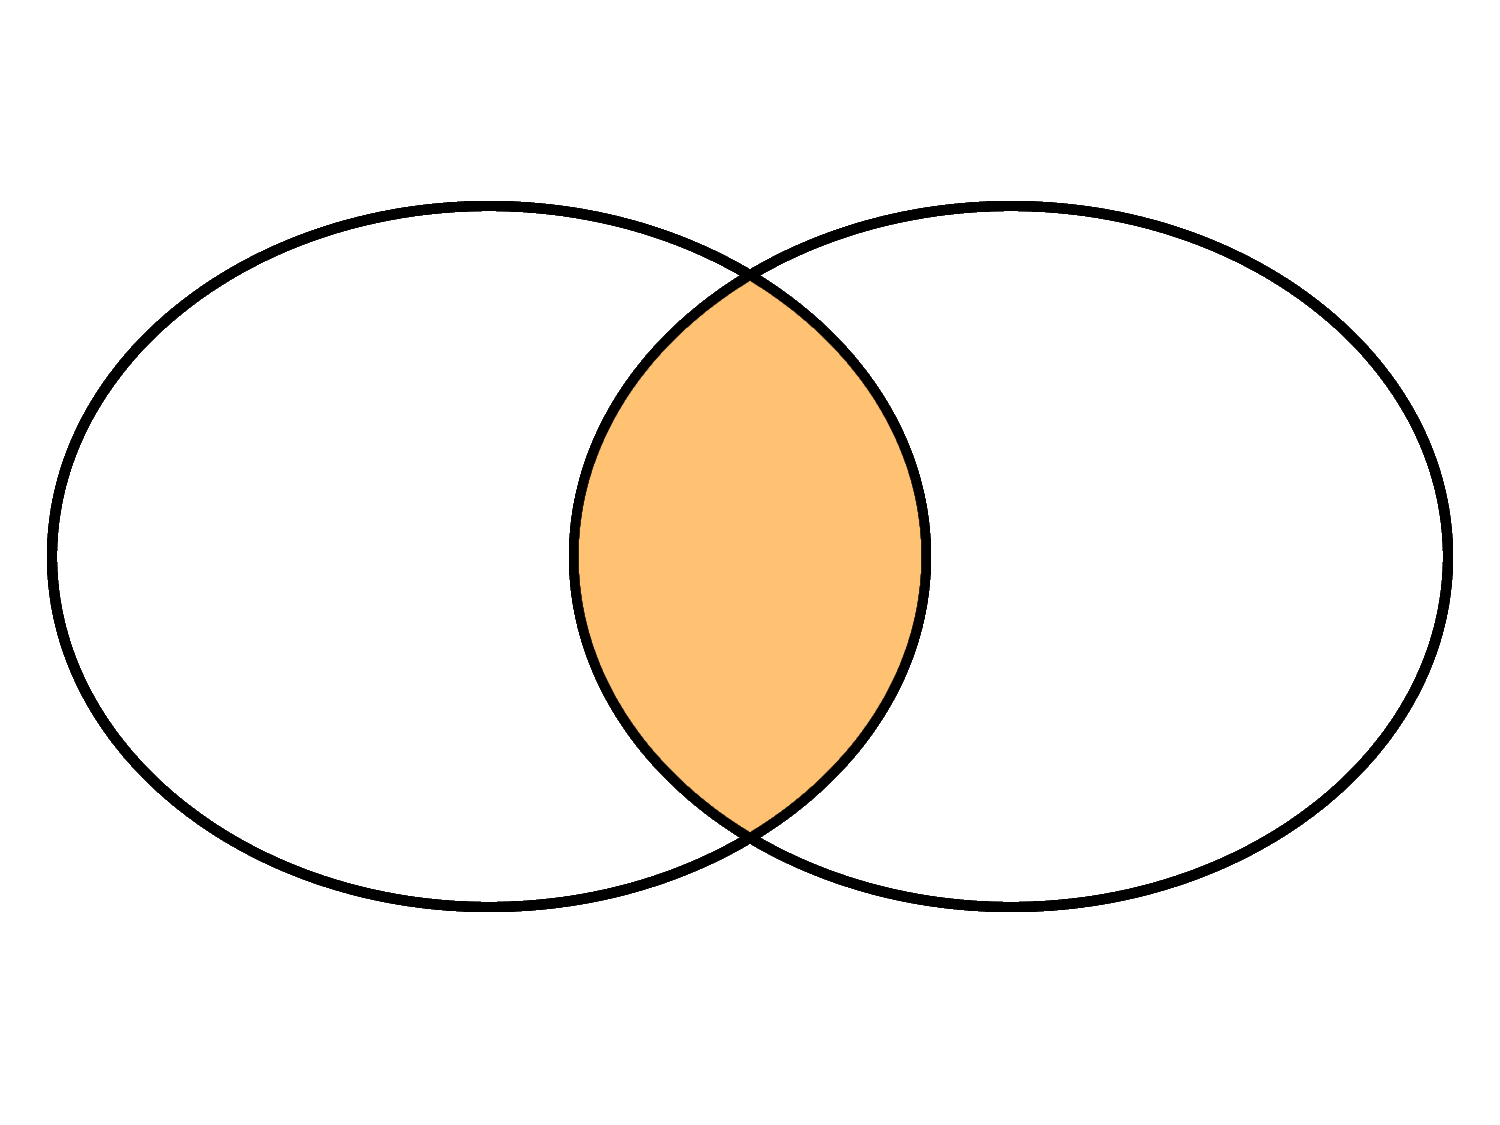
\includegraphics[width=0.7\textwidth]{../figures/AundB.png}
            \caption{Veranschaulichung der Schnittmenge}
            \label{fig:my_label}
        \end{figure}
    \end{columns}
\end{frame}

\begin{frame}{Mengenoperationen - Vereinigung}
    \begin{columns}
        \column{0.5\textwidth}
        \begin{alertblock}{Vereinigung - $A\cup B$}
            Gegeben zwei Mengen A und B.\\
            In der Vereinigung liegt alles, das nur in A, nur in B \textbf{oder} in beiden Mengen liegt.
        \end{alertblock}
        \column{0.5\textwidth}
        \begin{figure}
            \centering
            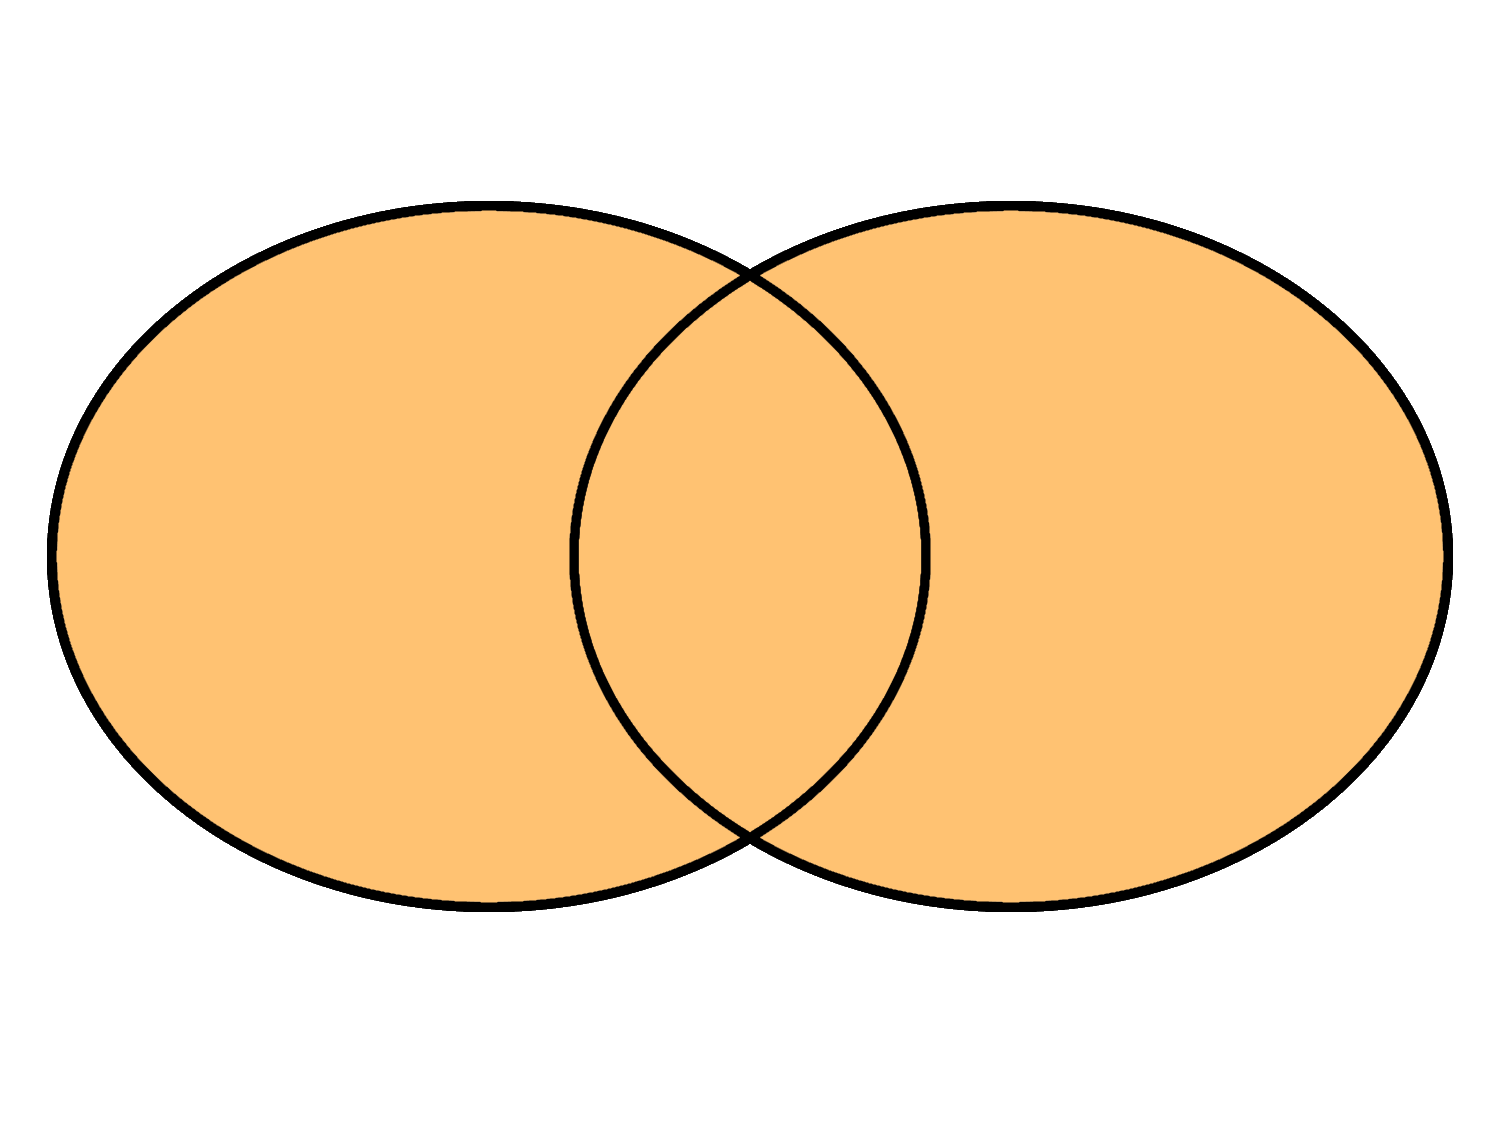
\includegraphics[width=0.7\textwidth]{../figures/AoderB.png}
            \caption{Veranschaulichung der Vereinigung}
            \label{fig:my_label}
        \end{figure}
    \end{columns}
\end{frame}

\begin{frame}{Mengenoperationen - Komplement}
    \begin{columns}
        \column{0.5\textwidth}
        \begin{alertblock}{Komplement - $\overline{A}$}
            Gegeben sei eine Menge A.\\
            Im Komplement der Menge A liegen alle Elemente, die in der Obermenge (z.B. $\mathbb{N}$), aber nicht in der Menge A selbst liegen.
        \end{alertblock}
        \column{0.5\textwidth}
        \begin{figure}
            \centering
            \begin{tikzpicture}[align=center]
    \node[
        ellipse, draw, minimum height = 2.5cm, minimum width = 4cm, fill = orange!45!white, line width = 0.25mm
    ] at (0,0) {$\overline{A}$};
    \node[
        ellipse, draw, minimum height = 1.2 cm, minimum width = 1.2cm, fill = white, line width = 0.25mm
    ] at (1cm,0) {$A$};
    \node[] at (2cm, -1cm) {$\mathbb{N}$};
\end{tikzpicture}
            \caption{Veranschaulichung des Komplements}
            \label{fig:komplement}
        \end{figure}
    \end{columns}
    \onslide<2>{\alert{\emph{Anmerkung:}} Kann auch geschrieben werden als $\mathbb{N}\setminus A$. \\
        \hspace{2cm}(gesprochen $\mathbb{N}$ \emph{\glqq ohne\grqq} $A$)}
\end{frame}

{\setbeamercolor{palette primary}{bg=ExColor}
\begin{frame}{Mengenoperationen}
    Berechne folgende Mengen
    \metroset{block=fill}
    \begin{alertblock}{Normal}
        \begin{itemize}
            \item $M_1 = \{1\}\cup \{2\}$
            \item $M_2 = \{\} \cap \{-1, 0, 1\}$
            \item $M_3 = \mathbb{N} \cup \mathbb{Z}$
            \item $M_4 = \overline{\{3^{n}\mid n \ \text{ist gerade}\} }$ über $\{3^{n}\mid n \in \mathbb{N}\}$
        \end{itemize}
    \end{alertblock}
    \begin{alertblock}{Schwer bis sehr schwer}
        \begin{itemize}
            \item $M_5 = \{1, 2, 3\} \cap  \{1, \{2, 3\}\}$
            \item $M_6 = \{u \mid |u| \equiv 0 \pmod 2, u \in \mathbb{N}\}$\\\hspace{0.65cm}$\cup$ $\{v \mid |v| \equiv 0 \pmod 4, v \in \mathbb{N}\}$
            \item $M_7 = \overline{\{a^{n} \mid n \ \text{ist gerade}, a \in \{3,4\}\}}$ über $\mathbb{N}$
        \end{itemize}
    \end{alertblock}
\end{frame}

\begin{frame}<handout:0>{Lösungen}
    \begin{itemize}[<+- | alert@+>]
        \item
              $M_1 = \{1, 2\}$
        \item
              $M_2 = \emptyset$
        \item
              $M_3 = \mathbb{Z}$
        \item
              $M_4 = \{3^{n} \mid$ n ist ungerade$\}$
        \item
              $M_5 = \{1\}$
        \item
              $M_6 = \{u \mid |u| \equiv 0 \pmod 2, u \in \mathbb{N}\}$
        \item
              $M_7 = \mathbb{N} \setminus \{9^n, 16^n \mid n \in \mathbb N\}$\\
              \hspace{0.44cm}$ = \mathbb{N} \setminus \{3^{2n}, 4^{2n} \mid n \in \mathbb N\}$
    \end{itemize}
\end{frame}
}


\metroset{sectionpage=progressbar,subsectionpage=none}

\section{Aussagenlogik}
\begin{frame}[fragile]{Was ist Aussagenlogik?}
    \begin{alertblock}{Aussagen}
    \begin{itemize}
        \item Paris ist die Hauptstadt von Frankreich
        \item Mäuse jagen Elefanten
        \item $5 \in \mathbb{N}$
        \item 5 = 8
        \item $u \in \{u, v, w\}$
    \end{itemize}
    \end{alertblock}
    Eine Aussage A ist entweder \textbf{wahr} oder \textbf{falsch}.
\end{frame}

\begin{frame}[fragile]{Was ist Aussagenlogik?}
    \begin{alertblock}{Das sind keine Aussagen}
    \begin{itemize}
        \item Macht theoretische Informatik Spaß?
        \item Geh dein Zimmer aufräumen!
        \item Wie viele Tiere wohnen in der Uni?
        \item $(x+y)^2+1$
        \item \{a,b,c\}
        \item ...
    \end{itemize}
    \end{alertblock}
    Diesen Sätzen können wir keinen eindeutigen Wahrheitswert \textbf{wahr} oder \textbf{falsch} zuordnen.
\end{frame}

\begin{frame}[fragile]{Was ist Aussagenlogik?}
    \begin{alertblock}{Wozu brauchen wir das?}
    \begin{itemize}
        \item Wir untersuchen, wie wir Aussagen verknüpfen können.
        \item Damit ziehen wir formale Schlüsse und führen Beweise.
    \end{itemize}
    \end{alertblock}
\end{frame}

\begin{frame}[fragile]{Logische Operationen}
Wir können Aussagen verändern oder durch Operationen zu neuen Aussagen verbinden.
\begin{itemize}
    \item A: Fred möchte Schokolade.
    \item B: Fred möchte Gummibärchen.
\end{itemize}
\metroset{block=fill}
\begin{alertblock}{Grundoperationen}
\begin{itemize}
    \item<1-> \textbf{Und}: A \alert<1>{$\wedge$} B $\leadsto$ Fred möchte Schokolade \alert<1>{und} Gummibärchen.\\
    \only<1>{\emph{Analog}: M: $M_1 \cap M_2$, Jedes Element aus M liegt in $M_1$ \textbf{und} in $M_2$}
    \item<2-> \textbf{Oder}: A \alert<2>{$\vee$} B $\leadsto$ Fred möchte Schokolade \alert<2>{oder} Gummibärchen.\\
    \only<2>{\emph{Anmerkung}: Inklusives \glqq oder\grqq, kein \glqq entweder oder\grqq \\
    Das heißt, es können auch beide Aussagen wahr sein.\\}
	\only<2>{\emph{Analog}: M: $M_1 \cup M_2$, Jedes Element aus M liegt in $M_1$ \textbf{oder} in $M_2$}
    \item<3> \textbf{Nicht}: \alert<3>{$\neg$}A $\leadsto$ Fred möchte \alert<3>{keine} Schokolade.\\
    \only<3>{\emph{Analog}: M: $\overline{M_1}$, Jedes Element aus M liegt \textbf{nicht} in $M_1$}
\end{itemize}
\end{alertblock}
\end{frame}


\begin{frame}{Überblick: Mengenoperationen}
	
	Auf \alert{Mengen} A, B lassen sich verschiedene Mengenoperationen ausführen.
	
	\metroset{block=fill}
	\begin{exampleblock}{Mengenoperationen}
		\begin{itemize}
			\item Schnitt: $A \cap B$
			\item Vereinigung: $A \cup B$
			\item Komplement: $\overline{A}$
		\end{itemize}
	\end{exampleblock}
\end{frame}

\begin{frame}{Überblick: Logische Operationen}
	
	Auf \alert{Aussagen} A, B lassen sich verschiedene logische Operationen ausführen.
	
	\metroset{block=fill}
	\begin{exampleblock}{Logische Operationen}
		\begin{itemize}
			\item Logisches Und: $A \wedge B$
			\item Logisches Oder: $A \vee B$
			\item Logisches Nicht: $\neg A$
		\end{itemize}
	\end{exampleblock}
\end{frame}

{\setbeamercolor{palette primary}{bg=ExColor}
	\begin{frame}{Logische Operationen vs. Mengenoperationen}
		\alert{Mengenoperationen und logische Operationen dürfen nicht verwechselt werden.}
		\begin{table}[]
			\begin{tabular}{l l}
				A: $5 \in \mathbb{N}$ & B: Es regnet\\
				C: \{$w \mid |w|=2$ \} \ & D: \{a,b,c,x,y\}\\
			\end{tabular}
		\end{table}
		\metroset{block=fill}
		\metroset{block=fill}
		\begin{block}{Welche dieser Verknüpfungen sind zulässig?}
			\begin{itemize}
				\item $L_1: A \wedge B$
				\item $L_2: A \vee C$
				\item $L_3: C \cap D$
				\item $L_4: A \wedge B \cup C$
			\end{itemize}
		\end{block}
	\end{frame}
}

{\setbeamercolor{palette primary}{bg=ExColor}
	\begin{frame}[fragile]{Logische Operationen vs. Mengenoperationen}
		\begin{itemize}[<+- | alert@+>]
			\item $L_1$: Zulässig
			\item $L_2$: Nicht zulässig
			\item $L_3$: Zulässig
			\item $L_4$: Nicht zulässig
		\end{itemize}
	\end{frame}
}



\begin{frame}{Logische Operationen: Implikation}
\begin{alertblock}{A$\implies$B}
\begin{itemize}
    \item \glqq Wenn A wahr ist, dann muss auch B wahr sein.\grqq
    \item kurz: \glqq\textbf{Wenn} A, \textbf{dann} B.\grqq
    \item Wenn A falsch ist können wir keine Aussage über B treffen.
    \item A$\implies$B ist dieselbe Aussage wie $\neg A \vee B$
\end{itemize}
\end{alertblock}
\end{frame}

\begin{frame}{Logische Operationen: Äquivalenz}
\begin{alertblock}{A$\iff$B}
\begin{itemize}
    \item \glqq A ist wahr, \textbf{genau dann wenn} B wahr ist.\grqq
    \item kurz: \glqq A gdw. B\grqq
    \item A und B müssen den selben Wahrheitswert haben.
    \item A$\iff$B ist dieselbe Aussage wie $(A \implies B) \wedge (B \implies A)$
\end{itemize}
\end{alertblock}
\end{frame}

{\setbeamercolor{palette primary}{bg=ExColor}
\begin{frame}[fragile]{Denkpause}
    \begin{alertblock}{Aufgaben}
      Berechne den Wahrheitswert folgender Aussagen. 
    \end{alertblock}
    \metroset{block=fill}
    \begin{block}{Normal}
    \begin{itemize}
        \item $A_1$: $5 \in \mathbb{N} \wedge a \in \{a, b, c\}$
        \item $A_2$: $0 \in \mathbb{N} \vee a \in \{a, b, c, d\}$
        \item $A_3$: $A_1 \iff A_2$
    \end{itemize}
    \end{block}
    \begin{block}{Etwas Schwerer}
    \begin{itemize}
        \item $A_4$: $(\emptyset=\emptyset^{*}) \implies (a \in \emptyset)$
        \item $A_5$: $(a \notin \emptyset) \implies (\emptyset = \emptyset^{*})$
        \item $A_6$: $A_4 \iff A_5$
        \item $A_7$: $(7 \in \{1, 2, 7, 9\}) \cap (2 = 7-5)$
        \item $A_8$: Wenn mein Auto fliegt, dann hast du auch ein fliegendes Auto.
    \end{itemize}
    \end{block}
\end{frame}
}

% {\setbeamercolor{palette primary}{bg=ExColor}
% \begin{frame}[fragile]{Denkpause}
%     \begin{alertblock}{Aufgaben}
%       Löse folgende Zusatzaufgabe. 
%     \end{alertblock}
%     \metroset{block=fill}
%     \begin{block}{Zusatz}
%     \begin{itemize}
%         \item $A_8$: Gegeben zwei Aussagen A, B.\\
%         Formuliere die Aussage $A \iff B$ nur unter Verwendung der Junktoren $\wedge, \vee, \neg$
%     \end{itemize}
%     \end{block}
% \end{frame}
% }

{\setbeamercolor{palette primary}{bg=ExColor}
\begin{frame}{Lösungen}
  \begin{itemize}[<+- | alert@+>]
        \item 
            $A_1$: wahr
        \item
            $A_2$: wahr
        \item
            $A_3$: wahr
        \item
            $A_4$: wahr 
        \item
            $A_5$: falsch
       	\item
       		$A_6$: falsch
        \item
            $A_7$: Das ist keine Aussage, da der Schnitt($\cap$) verwendet wurde um zwei Aussagen miteinander zu verknüpfen
       	\item
       		$A_8$: wahr
    \end{itemize}
\end{frame}
}

\begin{frame}[standout]
    Murmelpause
\end{frame}

% {\setbeamercolor{palette primary}{bg=ExColor}
% \begin{frame}{Lösungen}
%     \metroset{block=fill}
%     \begin{block}{Zusatz}
%     \begin{itemize}
%         \item $A_8$: Gegeben zwei Aussagen A, B.\\
%         Formuliere die Aussage $A \iff B$ nur unter Verwendung der Junktoren $\wedge, \vee, \neg$
%     \end{itemize}
%     \end{block}
%   \begin{alertblock}{Lösung}
%         \begin{itemize}[<+- | alert@+>]
%             \item Äquivalenz bedeutet intuitiv: Beide wahr oder beide falsch
%             \item $A_8$: $(A \wedge B) \vee (\neg A \wedge \neg B)$
%         \end{itemize}
%   \end{alertblock}
% \end{frame}
% }




\begin{frame}{Anwendung der Implikation}
    Wir haben zwei Aussagen $A$ und $B$. Wir nehmen nun an, $A$ sei wahr. Wenn wir zeigen, dass dann auch $B$ wahr ist, wissen wir, dass $A \implies B$ gilt.
\metroset{block=fill}
\begin{exampleblock}{Beispiel}
\begin{enumerate}
    \item<1-> Wir wollen zeigen, dass für eine ganze Zahl $x$ \\
    die Implikation $3 = x - 2 \implies x = 5$ gilt.
    \item<2-> Wir nehmen an, dass die linke Aussage wahr ist\dots
    \item<3-> \dots und zeigen, dass dann die rechte Aussage gilt.
    \item<4-> $(3 = x - 2) \implies (3 + 2 = x) \implies (5 = x) \implies (x = 5)$
    \item<5-> Also folgt die rechte Aussage aus der linken
    \item<6-> Somit gilt die Implikation \qed\;
\end{enumerate}
\end{exampleblock}
\end{frame}

% {\setbeamercolor{palette primary}{bg=ExColor}
% \begin{frame}{Denkpause}
%     \begin{alertblock}{Aufgaben}
%       Welche der folgenden Schlüsse sind richtig? 
%     \end{alertblock}
%     \metroset{block=fill}
%     \begin{block}{Normal bis Schwer}
%     \begin{itemize}
%         \item $S_1$: Lukas ist im Vorkurs oder schläft noch. Im Vorkurs ist er nicht. Also schläft er noch.
%         \item $S_2$: Wenn Anne nicht rennt, bekommt sie die Bahn nicht. Sie bekommt die Bahn. Also ist sie gerannt.
%         \item $S_3$: Wenn Tobi nicht lernt, besteht er nicht. Tobi hat gelernt. Also besteht er.
%     \end{itemize}
%     \end{block}
% \end{frame}
% }

% {\setbeamercolor{palette primary}{bg=ExColor}
% \begin{frame}{Lösungen}
%   \begin{itemize}[<+- | alert@+>]
%         \item 
%             $S_1$: Richtig.
%         \item
%             $S_2$: Richtig. Begründung: Die zweite Aussage ist die Kontraposition der ersten Aussage. Wie gezeigt wurde, ist die Kontraposition einer Aussage wahr gdw. die Aussage selbst wahr ist.
%         \item
%             $S_3$: Falsch. Beispiel: Tobi lernt, und besteht trotzdem nicht. \Frowny
%     \end{itemize}
% \end{frame}
% }


\section{Quantoren}
\begin{frame}[fragile]{Quantoren}
    Oft wollen wir Aussagen nicht nur für ein Element, sondern für viele Elemente treffen.
    \metroset{block=fill}
    \begin{exampleblock}{Beispiel}
        $A_1$: Für die Zahl 5 gilt: Sie hat einen Nachfolger\\
        \emph{Allgemeiner:}\\
        $A_2$: Für jede natürliche Zahl n gilt: n hat einen Nachfolger
    \end{exampleblock}
    \begin{exampleblock}{Beispiel}
        $A_3$: Für die Zahl 5 gilt: Sie ist eine Primzahl\\
        \emph{Allgemeiner:}\\
        $A_4$: Es gibt eine natürliche Zahl n, so dass gilt: n ist eine Primzahl
    \end{exampleblock}
\end{frame}

\begin{frame}[fragile]{Quantoren}
    Mithilfe von \textbf{Quantoren} vereinfachen wir uns die Schreibweise dieser Aussagen.\\
    \vspace{0.5cm}
    Quantor \alert{$\forall$}: Die Aussage gilt für alle Elemente.\\
    \metroset{block=fill}
    \begin{exampleblock}{Beispiel}
        $A_1$: $\forall k \in \mathbb{N}:$ 2k ist gerade
    \end{exampleblock}
    Quantor \alert{$\exists$}: Die Aussage gilt für mindestens ein Element.\\
    \metroset{block=fill}
    \begin{exampleblock}{Beispiel}
        $A_2$: $\exists k \in \mathbb{N}:$ k ist Primzahl
    \end{exampleblock}
\end{frame}

\begin{frame}[fragile]{Quantoren}
    In einer Aussage können mehrere Quantoren vorkommen.\\
    Wir lesen dann von links nach rechts.
    \metroset{block=fill}
    \begin{exampleblock}{Beispiel}
        $A_1$: $\forall x,y \in \mathbb{N}: \exists z \in \mathbb{N}: x+y = z$\\
        Bedeutung: Für zwei beliebige Zahlen x und y aus $\mathbb{N}$ gibt es eine weitere natürliche Zahl z, so dass $x+y=z$ gilt.
    \end{exampleblock}
\end{frame}

\begin{frame}[fragile]{Quantoren}
    \alert{Achtung!}\\
    Die Reihenfolge von zwei Quantoren zu vertauschen, kann die Bedeutung einer Aussage deutlich verändern.
    \metroset{block=fill}
    \begin{exampleblock}{Beispiel}
        x,y $\in$ Studenten\\
        \textbf{$A_1$: $\forall x \exists y:$ x schlägt y\\
        $A_2$: $\exists x \forall y:$ x schlägt y\\ }
        Was ist der Unterschied zwischen beiden Aussagen?
    \end{exampleblock}
\end{frame}

\begin{frame}{Quantoren}
    \begin{alertblock}{Aufgabe}
      Wir formulieren folgende Aussage mithilfe von Quantoren und den Symbolen der Aussagenlogik (Junktoren).
    \end{alertblock}
    \metroset{block=fill}
    \begin{block}{Beispiel}
    \begin{itemize}
        \item $A_1$: Eine ganze Zahl ist eine natürliche Zahl, wenn sie positiv oder null ist.
    \end{itemize}
    \end{block}
    \begin{block}{Hinführung}
    \begin{itemize}
        \item $A_1$: Für alle ganzen Zahlen x gilt: Wenn x positiv oder null ist, ist x eine natürliche Zahl.
    \end{itemize}
    \end{block}
    \begin{block}{\alert{Lösung}}
    \begin{itemize}
        \item $A_1$: $\forall x \in \mathbb{Z}: x \geq 0 \implies x \in \mathbb{N}$
    \end{itemize}
    \end{block}
\end{frame}

{\setbeamercolor{palette primary}{bg=ExColor}
\begin{frame}{Denkpause}
    \begin{alertblock}{Aufgaben}
      Formuliere folgende Aussagen mithilfe von Quantoren und den Symbolen der Aussagenlogik (Junktoren). 
    \end{alertblock}
    \metroset{block=fill}
    \begin{block}{Normal}
    \begin{itemize}
        \item $A_1$: Die Differenz zweier ganzer Zahlen ist wieder eine ganze Zahl.
    \end{itemize}
    \end{block}
    \begin{block}{Schwer}
    \begin{itemize}
        \item $A_2$: Jede natürliche Zahl lässt sich als Summe von vier Quadratzahlen darstellen.
    \end{itemize}
    \end{block}
    \begin{block}{Da haben selbst wir keinen Bock drauf}
    \begin{itemize}
        \item $A_3$: Eine natürliche Zahl, die von einer von ihr verschiedenen natürlichen Zahl größer als 1 geteilt wird, ist nicht prim.
    \end{itemize}
    \end{block}
\end{frame}
}

{\setbeamercolor{palette primary}{bg=ExColor}
\begin{frame}{Lösungen}
  \begin{itemize}[<+- | alert@+>]
        \item 
            $A_1$: $\forall x,y \in \mathbb{Z}: x-y \in \mathbb{Z}$
        \item
            $A_2$: $\forall x \in \mathbb{N}: \exists a, b, c, d \in \mathbb{N}: x = a^2 + b^2 + c^2 + d^2$
        \item
            $A_3$: $\forall x \in \mathbb{N}: \left(\exists y \in \mathbb{N}: (y>1) \wedge (y \neq x) \wedge (y \mid x)\right) \implies x\ \text{ist keine Primzahl}$.
    \end{itemize}
\end{frame}
}

\begin{frame}[fragile]{Äquivalente Schreibweisen von Mengenoperationen}
	Oft benötigen wir eine Aussagenlogische Äquivalente Bedingung von Mengenoperationen.
	\metroset{block=fill}
	\begin{block}{Operationen}
		\begin{itemize}
			\item<1-> \textbf{Teilmenge}: A \alert<1>{$\subseteq$} B $\leadsto$ $\forall x \in A: x \in B$\\
			\item<2-> \textbf{Vereinigung}: C = A \alert<2>{$\cup$} B $\leadsto$ $\forall x \in C: x \in A \vee x \in B$\\
			\item<3-> \textbf{Schnitt}: C = A \alert<3>{$\cap$} B $\leadsto$ $\forall x \in C: x \in A \wedge x \in B$\\
			\item<4-> \textbf{Komplement}: \alert<4>{$\overline{A}$} $\leadsto$ $\forall x \in \overline{A}: x \notin A$
		\end{itemize}
	\end{block}
	
\end{frame}


\section{Beweisen}
% Copyright 2018, 2019, 2020, 2021 FIUS
%
% This file is part of theo-vorkurs-folien.
%
% theo-vorkurs-folien is free software: you can redistribute it and/or modify
% it under the terms of the GNU General Public License as published by
% the Free Software Foundation, either version 3 of the License, or
% (at your option) any later version.
%
% theo-vorkurs-folien is distributed in the hope that it will be useful,
% but WITHOUT ANY WARRANTY; without even the implied warranty of
% MERCHANTABILITY or FITNESS FOR A PARTICULAR PURPOSE.  See the
% GNU General Public License for more details.
%
% You should have received a copy of the GNU General Public License
% along with theo-vorkurs-folien.  If not, see <https://www.gnu.org/licenses/>.

\begin{frame}{Einführung}
\begin{alertblock}{Was ist ein Beweis?}
\begin{itemize}
        \item lückenlose Folge von logischen Schlüssen,\\welche zur zu beweisenden Behauptung führen
        \item nicht nur einleuchtend, sondern zweifelsfrei korrekt
    \end{itemize}
\end{alertblock}
\end{frame}

\subsubsection{Beweisbeispiel: Transitivität der Teilmenge}
\begin{frame}[fragile]{Beispielbeweis}
\begin{exampleblock}{Zu zeigen: Teilmengen sind transitiv.}
\begin{enumerate}
    \item<1->\alert<1|handout:0>{
        \only<1|handout:0>{zu zeigen: }\onslide<2->{z.z. }$A\subseteq B\wedge B\subseteq C \alert<3|handout:0>{\implies\text{}}A\subseteq C$
        }
    \item<2->\alert<2|handout:0>{
        \only<2|handout:0>{Umschreiben:\\}
        $\iff $\alert<4,5|handout:0>{$($\alert<9|handout:0>{$($\alert<6|handout:0>{$\forall x$}$\ : x \in A \implies x \in B)$}$ \wedge $\alert<10|handout:0>{$($\alert<6|handout:0>{$\forall x$}$\ : x \in B \implies x \in C)$}$)$}\\
        \qquad\alert<3|handout:0>{$\implies$}$\;($\alert<6|handout:0>{$\forall x$}$\ :\ $\alert<7|handout:0>{$x \in A$}$ \implies x \in C)$
        }
    \item<3->\alert<3|handout:0>{
        \only<3|handout:0>{\emph{Implikation}\\
        linke Seite wahr $\implies$ rechte Seite muss wahr sein.\\
        linke Seite falsch $\implies$ beliebiges kann folgen\\
        $\implies$ uns interessiert also nur der Fall \emph{links ist wahr}}
        \alert<4>{\only<4,5|handout:0>{Wir machen uns also \emph{\textquotedbl die linke Seite ist wahr\textquotedbl} zur Voraussetzung}\alert<5>{\only<5|handout:0>{:\\Angenommen, $A \subseteq B \wedge B \subseteq C$ gilt.}}}
        \onslide<6->{Ang., $A \subseteq B \wedge B \subseteq C$.}
        }
    \item<6->\alert<6|handout:0>{
        \only<6|handout:0>{Jetzt geht der Beweis richtig los.\\Wähle beliebiges $x$, um Allgemeinheit zu wahren\dots\\}
        \onslide<6->{Sei $x$ beliebig}\alert<7>{\onslide<7-|handout:0>{, mit \alert<9>{$x\in A$.}}}
        }
    \item<8->\alert<8-9|handout:0>{
        \only<8|handout:0>{Wir können jetzt unsere Voraussetzungen ausnutzen,\\um $x\in C$ zu folgern.}
        \onslide<9->$\implies x\in B$
        \alert<10|handout:0>{\onslide<10->$\implies x\in C$}
        \onslide<11>\qed
    }
  \end{enumerate}
\end{exampleblock}
\end{frame}


\section{Wiederholung}
\begin{frame}[fragile]{Das können wir jetzt beantworten}
	\begin{alertblock}{Einführung}
		\begin{itemize}
			\item Theoretische Informatik ist ganz schön wichtig...
			\item ...für mein Studium.
		\end{itemize}
	\end{alertblock}
\end{frame}

\begin{frame}[fragile]{Das können wir jetzt beantworten}
	\begin{alertblock}{Mengen, Sprachen, Elemente}
		\begin{itemize}
			\item Was ist eine Menge?
			\item Was ist eine Sprache?
			\item Was sind Elemente einer Sprache/Menge?
		\end{itemize}
	\end{alertblock}
\end{frame}

\begin{frame}[fragile]{Das können wir jetzt beantworten}
	\begin{alertblock}{Operationen auf Mengen}
		\begin{itemize}
			\item Wie funktionieren Vereinigung, Schnitt und Komplement?
			\item Wie bilde ich die Vereinigung oder Schnittmenge zweier Mengen?
			\item Wie bilde ich das Komplement einer Menge?
			\item Wie kann ich Sprachen formal beschreiben?
			\item Hantieren mit verschiedenen seltsamen Mengen und den Verknüpfungen
		\end{itemize}
	\end{alertblock}
\end{frame}
\begin{frame}[fragile]{Das können wir jetzt beantworten}
	\begin{alertblock}{Logik}
		\begin{itemize}
			\item Was ist eine Aussage?
			\item Was bedeuten $\wedge$, $\vee$ und $\neg$?
			\item Wie funktioniert die Implikation?
			\item Wie funktioniert die Äquivalenz?
		\end{itemize}
	\end{alertblock}
\end{frame}
\begin{frame}[fragile]{Glossar \textemdash\ Quantoren}
    \small
    \begin{tabular}{p{0.33\textwidth} p{0.2\textwidth} p{0.45\textwidth}}
        \toprule
        Abk.                         & Bedeutung                                        & Was?!                                                              \\
        \midrule
        $\forall x \in M : A(x)$     & Für alle $x$ aus $M$ gilt $A(x)$                 & Die Aussage $A$ muss für alle Elemente der Menge $M$ wahr sein     \\
        $\exists x \in M : A(x)$     & Es existiert ein $x$ in $M$ für das $A(x)$ gilt  & Die Aussage $A(x)$ muss für mind. 1 (oder mehr) Elemente wahr sein \\
        $\forall x,y \in M : A(x,y)$ & Für alle $x$ \textit{und} alle $y$ gilt $A(x,y)$ & Äquivalent zu $\forall x \forall y : A(x,y)$                       \\
        \bottomrule
    \end{tabular}
\end{frame}
% Copyright 2018, 2019, 2020, 2021 FIUS
%
% This file is part of theo-vorkurs-folien.
%
% theo-vorkurs-folien is free software: you can redistribute it and/or modify
% it under the terms of the GNU General Public License as published by
% the Free Software Foundation, either version 3 of the License, or
% (at your option) any later version.
%
% theo-vorkurs-folien is distributed in the hope that it will be useful,
% but WITHOUT ANY WARRANTY; without even the implied warranty of
% MERCHANTABILITY or FITNESS FOR A PARTICULAR PURPOSE.  See the
% GNU General Public License for more details.
%
% You should have received a copy of the GNU General Public License
% along with theo-vorkurs-folien.  If not, see <https://www.gnu.org/licenses/>.

\begin{frame}{Einführung}
\begin{alertblock}{Was ist ein Beweis?}
\begin{itemize}
        \item lückenlose Folge von logischen Schlüssen,\\welche zur zu beweisenden Behauptung führen
        \item nicht nur einleuchtend, sondern zweifelsfrei korrekt
    \end{itemize}
\end{alertblock}
\end{frame}

\subsubsection{Beweisbeispiel: Transitivität der Teilmenge}
\begin{frame}[fragile]{Beispielbeweis}
\begin{exampleblock}{Zu zeigen: Teilmengen sind transitiv.}
\begin{enumerate}
    \item<1->\alert<1|handout:0>{
        \only<1|handout:0>{zu zeigen: }\onslide<2->{z.z. }$A\subseteq B\wedge B\subseteq C \alert<3|handout:0>{\implies\text{}}A\subseteq C$
        }
    \item<2->\alert<2|handout:0>{
        \only<2|handout:0>{Umschreiben:\\}
        $\iff $\alert<4,5|handout:0>{$($\alert<9|handout:0>{$($\alert<6|handout:0>{$\forall x$}$\ : x \in A \implies x \in B)$}$ \wedge $\alert<10|handout:0>{$($\alert<6|handout:0>{$\forall x$}$\ : x \in B \implies x \in C)$}$)$}\\
        \qquad\alert<3|handout:0>{$\implies$}$\;($\alert<6|handout:0>{$\forall x$}$\ :\ $\alert<7|handout:0>{$x \in A$}$ \implies x \in C)$
        }
    \item<3->\alert<3|handout:0>{
        \only<3|handout:0>{\emph{Implikation}\\
        linke Seite wahr $\implies$ rechte Seite muss wahr sein.\\
        linke Seite falsch $\implies$ beliebiges kann folgen\\
        $\implies$ uns interessiert also nur der Fall \emph{links ist wahr}}
        \alert<4>{\only<4,5|handout:0>{Wir machen uns also \emph{\textquotedbl die linke Seite ist wahr\textquotedbl} zur Voraussetzung}\alert<5>{\only<5|handout:0>{:\\Angenommen, $A \subseteq B \wedge B \subseteq C$ gilt.}}}
        \onslide<6->{Ang., $A \subseteq B \wedge B \subseteq C$.}
        }
    \item<6->\alert<6|handout:0>{
        \only<6|handout:0>{Jetzt geht der Beweis richtig los.\\Wähle beliebiges $x$, um Allgemeinheit zu wahren\dots\\}
        \onslide<6->{Sei $x$ beliebig}\alert<7>{\onslide<7-|handout:0>{, mit \alert<9>{$x\in A$.}}}
        }
    \item<8->\alert<8-9|handout:0>{
        \only<8|handout:0>{Wir können jetzt unsere Voraussetzungen ausnutzen,\\um $x\in C$ zu folgern.}
        \onslide<9->$\implies x\in B$
        \alert<10|handout:0>{\onslide<10->$\implies x\in C$}
        \onslide<11>\qed
    }
  \end{enumerate}
\end{exampleblock}
\end{frame}


\Center{Noch Fragen?}

\begin{frame}[fragile]{Das können wir jetzt beantworten}
	\begin{alertblock}{Mengen, Sprachen, Elemente}
		\begin{itemize}
			\item Was ist eine Menge?
			\item Was ist eine Sprache?
			\item Was sind Elemente einer Sprache/Menge?
		\end{itemize}
	\end{alertblock}
\end{frame}

\begin{frame}[fragile]{Das können wir jetzt beantworten}
	\begin{alertblock}{Operationen auf Mengen}
		\begin{itemize}
			\item Wie funktionieren Vereinigung, Schnitt und Komplement?
			\item Wie bilde ich die Vereinigung oder Schnittmenge zweier Mengen?
			\item Wie bilde ich das Komplement einer Menge?
			\item Wie kann ich Sprachen formal beschreiben?
			\item Hantieren mit verschiedenen seltsamen Mengen und den Verknüpfungen
		\end{itemize}
	\end{alertblock}
\end{frame}
\begin{frame}[fragile]{Glossar - Aussagenlogik}
    \small
    \begin{tabular}{p{0.33\textwidth} p{0.2\textwidth} p{0.45\textwidth}}
        \toprule
        Abk.                     & Bedeutung                                       & Was?!                                                              \\
        \midrule
        $A\land B$               & A \textit{und} B                                & A und B müssen wahr sein, damit die Gesamtaussage wahr ist         \\
        $A\lor B$                & A \textit{oder} B                               & Es müssen mindestend A, B oder beide wahr sein                     \\
        $\lnot A$                & \textit{nicht} A                                & A muss falsch sein, damit $\lnot A$ wahr ist                       \\
        $B \implies B$           & A ist notwendig für B                           & A muss wahr sein, wenn B wahr ist                                  \\
        $A \implies B$           & A ist hinreichend für / impliziert B            & B muss wahr sein, wenn A wahr ist                                  \\
        $A \iff B$               & notwendig und hinreichend                       & genau dann, wenn                                                   \\
        $\forall x \in M : A(x)$ & Für alle $x$ aus $M$ gilt $A(x)$                & Die Aussage $A$ muss für alle Elemente der Menge $M$ wahr sein     \\
        $\exists x \in M : A(x)$ & Es existiert ein $x$ in $M$ für das $A(x)$ gilt & Die Aussage $A(x)$ muss für mind. 1 (oder mehr) Elemente wahr sein \\
        \bottomrule
    \end{tabular}
\end{frame}

\appendix
% Copyright 2018-2022 FIUS
%
% This file is part of theo-vorkurs-folien.
%
% theo-vorkurs-folien is free software: you can redistribute it and/or modify
% it under the terms of the GNU General Public License as published by
% the Free Software Foundation, either version 3 of the License, or
% (at your option) any later version.
%
% theo-vorkurs-folien is distributed in the hope that it will be useful,
% but WITHOUT ANY WARRANTY; without even the implied warranty of
% MERCHANTABILITY or FITNESS FOR A PARTICULAR PURPOSE.  See the
% GNU General Public License for more details.
%
% You should have received a copy of the GNU General Public License
% along with theo-vorkurs-folien.  If not, see <https://www.gnu.org/licenses/>.

\subsection{Lizenz}
\begin{frame}[fragile]{Lizenz}
    \begin{itemize}
    \item Unsere Folien sind frei!\\
    \item Jeder darf die Folien unter den Bedingungen der \textbf{GNU General Public License v3} (oder jeder späteren Version) weiterverwenden.\\
    \item Ihr findet den Quelltext unter \url{https://www.github.com/FIUS/theo-vorkurs-folien}
    \end{itemize}
\end{frame}
\begin{frame}<handout:0>[fragile]{Online-Whiteboard}
	\phantom{text}
\end{frame}

\end{document}
